\section{The Scratch Online Community}

%TODO: once settled with layout, make sure it does not use a full page just for this image
\begin{figure}
\centering
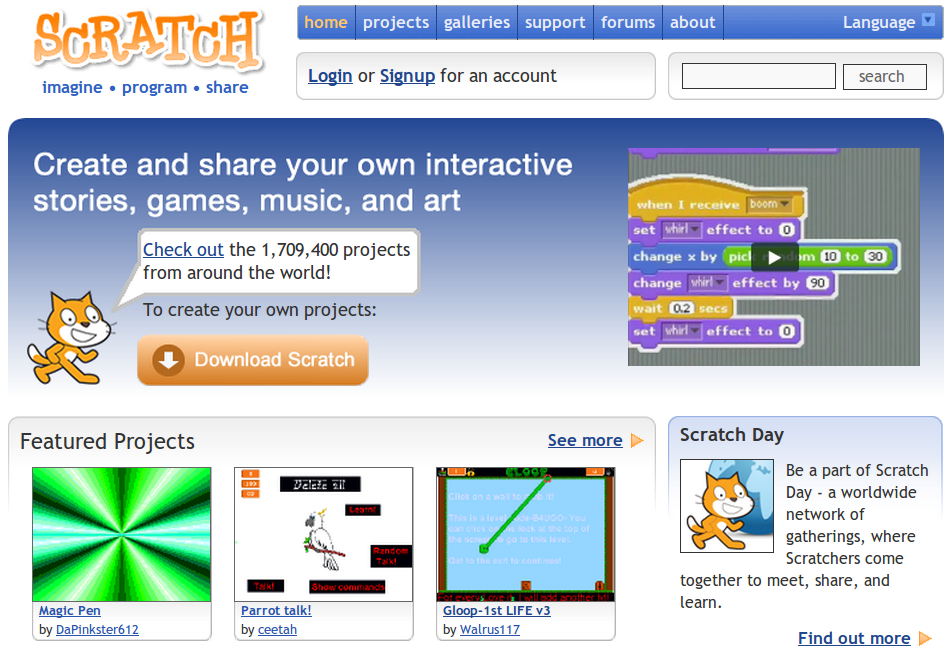
\includegraphics[width=3.25in]{figures/websitehomepage.png}
\caption{The home page of the Scratch website}
\label{fig:websitehomepage}
\end{figure}

The empirical setting for this work is the Scratch Online Community, a website (Figure~\ref{fig:websitehomepage}) I conceived and developed over the past four years in collaboration with others at the Lifelong Kindergarten research group, for this and other lines of research.
The website allows anyone, especially young people between ages eight and sixteen, to share their animated stories, interactive art, and video games. Participants use the Scratch programming environment, a desktop application, to create or remix projects by putting together images, music and sounds with visual programming command blocks \citep{resnick_scratch:_2009}.
Projects range from interactive greeting cards, physics simulations, animations of popular songs to homemade video games, just to name a few.  

Scratch projects are organized in sprites (e.g. a character in a game).
Each sprite has a set of ``costumes'' or images that represent its different visual states, for example, a sprite of a bird flying could have multiple costumes, each one representing the different positions of the wings. 
Sprites can also have sounds associated to them, these sounds can be either recorded with the microphone or imported from the hard creator's hard drive. Finally, sprites' behavior is controlled by ``scripts'' which are stacks of visual programming blocks. 

In my dissertation, I plan to document in detail the motivations that led to the design of the Scratch website as it is now and the various iterations that it went through as a result of internal and user-driven demands and participation patterns.
I expand on the tight relationship between the technical capabilities of the website and the social dynamics that it supported or intended to support.
I take a critical look at how the original goals of the community were or were not achieved and in what ways that happened. 
I narrate scalability challenges with the technology and moderation of the community.
In the following two sections I provide a glimpse of this.

More broadly, I try to tackle questions such as: How was the culture of sharing seeded and maintained in a public space? What were some important incidents that changed policies or architecture? How did the architecture and management of the site influence the culture of the site and how did users help shap this? 
Was it the design of the space or the work of users to create the culture?
 What were the lessons learned along the way by administrators? What kinds of learning outcomes were achieved?
To answer some of these questions, I primarily rely on participant observation data, experiences collected during the three years and I support these arguments with descriptive statistics and case studies.


\subsection{Motivations}

From its start \citep{monroy-hernandez_scratchr:_2007,monroy-hernandez_empowering_2008}, I set the goal for the Scratch Online Community as to give creators access to 
1) a \emph{network of peers} that functions as an audience and as potential collaborators and,
2) a \emph{repository} of inspirational creations that can be creatively appropriated by anyone.

More broadly, the Scratch Online Community was created with the idea of supporting a Community of Practice around Scratch where novices and experts would come together,  in the spirit of Papert's Samba school's metaphor \citep{papert_mindstorms_1980}.

Additionally, the idea of the Scratch Online Community was conceived under the umbrella of embodying the ethos of Participatory Culture of empowering people to become producers rather than just consumers of media.

Last, the Scratch Online Community was motivated to support the various iterative stages of the creative process \citep{resnick_sowing_2008}, namely:
Supporting creators' \emph{imagination} by giving access to a pool of inspirational projects and ideas; supporting \emph{creation} by allowing people to reuse and remix; supporting \emph{play} by letting people interact with others and their creations within a community; supporting \emph{sharing} by allowing people to easily upload their creations to the platform; supporting \emph{reflection} by providing a space to receive comments and discussion forums for more in-depth discussions.

\subsection{Sociotechnical Infrastructure}
The Scratch website platform, called ScratchR, is broadly composed of the following components: 

\begin{enumerate}
\item A repository of projects and metadata. Projects can be downloaded by anyone, modified and re-uploaded to the website as a remix. Each project has its web page where it is displayed and where people can interact with it and other people. 

\item A social network consisting of profile pages and unidirectional friendship connections. Profile pages list the friends, projects and ``favorited'' projects for each user with his or her avatar image and the Country of origin (all self-reported data).

\item Social features for interacting with people's creation such as commenting, tagging, ``loving'', ``favoriting''.

\item Galleries, which are pages where people can group projects and talk about them. It is important to note that galleries have been repurposed by the community as group spaces where people collaborate to create projects or use it as a space to talk to one another or play Role Playing Games.

\item Discussion forums where community members help one another with technical problems, find collaborators and talk about non-Scratch related activities that foster a sense of community on the website.

\item External services supported by an API\footnote{API stands for Application Program Interface. In ScratchR, they are a set of web-accessible functions that let people retrieve and submit data such as login authentication and information about projects.} such as a website where people can link projects or a Wiki where people can document their experiences with Scratch and the community.
\end{enumerate}

The website runs on a hybrid model for moderation that combines user-driven moderation through flagging and appointed moderators working in parallel with a full-time staff member and other part-time ones that review the flags and ensure that the social dynamics are kept as civil as possible. 
This model has allowed for scaling the community management at a relatively low cost, however, much of the architecture and software development during the three years has been put into mechanisms for preventing antisocial behavior.

Three years after its official release, the Scratch Online Community website I developed, handles more than ten million page views and six hundred-thousand people monthly.
This web traffic is more than half the page views of websites like newsweek.com\footnote{04/2011 data from http://www.quantcast.com/newsweek.com}.
As of April of 2011, more than 1.7 million projects have been uploaded at an average of 1 MB per project. 
Every second, the website receives up to 180 requests and it transfers 4MB.

To handle this level of activity, ScratchR, the website's underlying platform, uses a caching engine for static content called Varnish and another for dynamic content and database queries called Memcached. 
ScratchR runs on a completely Free and Open Source software stack that includes Apache for its web server and MySQL for its database running on CentOS Linux. 
ScratchR is written using a PHP-based framework called CakePHP.
Additionally, ScratchR supports external  web applications such as a discussion forum, a user-driven Wiki, a statistics visualization website, a Scratch sprites sharing website, and a few other websites that provide additional support to community members. 
These extra websites are supported through an API that has allowed scalability.
